
\chapter{Dendrite models}
\label{chap:dendrite-models}

\section{Dendritic conduction}
\label{sec:dendritic-conduction}


% \section{Introduction}
% \label{sec:introduction-7}

Let's review the cable equation
\begin{eqnarray}
  \label{eq:439}
    \frac{\partial V_m}{\partial T}  =
   \frac{\partial^2V_m}{\partial X^2} + f(V_m,T)
\end{eqnarray}

In axon, e.g.  squid giant axon, $f(V_m,T)$ in the formula by
Hodgkin-Huxley was a function of $m,n,h$ and $V_m$. This choice of $f$
allow the wave (action potential) propagated at a constant speed and
fixed profile, as shown in Fig.~\ref{fig:HH2}. This is called
{\it active waves} as it needs energy to maintain the necessary ionic
concentration.

In dendrite, the propagating is a passive activity, thus the
approximation $f=-V_m$ is valid. For simplicity, we shift $V$ so that
the resting potential is zero, i.e. $V=V_m-V_{rest}$. Thus, we have
\begin{eqnarray}
  \label{eq:438}
    \frac{\partial V}{\partial T}  =
   \frac{\partial^2V}{\partial X^2} - V
\end{eqnarray}
is called {\bf linear cable equation}.  In this form, the current
flows along the cable in a passive manner, leaking to the outside at a
linear rate. 

\section{Boundary condition}
\label{sec:boundary-condition}

To determine the behavior of a single dendrite, we need an initial
condition and a boundary condition.

Usually, it is assumed that at time $T=0$, the dendrite is at resting
state, $V_m=0$, thus
\begin{eqnarray}
  \label{eq:440}
  V_m(X,0) = 0
\end{eqnarray}

For boundary condition, suppose that $X=X_b$ is the boundary point,
then there are different to specify the boundary condition
\begin{enumerate}
\item Voltage-clamp boundary condition: 
  \begin{eqnarray}
    \label{eq:441}
    V(X_b,T) = V_b
  \end{eqnarray}
with $V_b$ is the voltage clamped (fixed) at $X=X_b$

\item Short circuit: at the end of the cable are short-circuited, thus
  the intracellular and extracellular are equal
  \begin{eqnarray}
    \label{eq:442}
    V(X_b,T) = V_b = V_i-V_e = 0
  \end{eqnarray}

\item Current injection: at the end of the cable, a current $I(T)$ is
  injected. As
  \begin{eqnarray}
    \label{eq:443}
    I_i = -\frac{1}{r_i}\frac{\partial V_i}{\partial x} =  -\frac{1}{r_i\lambda_m}\frac{\partial V_i}{\partial X}
  \end{eqnarray}
then
\begin{eqnarray}
  \label{eq:444}
  \frac{\partial V_m(X_b,T)}{\partial X} = -r_i\lambda_mI(T)
\end{eqnarray}
If $X_b$ is at the left end, this is an inward current, otherwise, it
is an outward current.

\item Sealed end: the end of the cable is sealed so that there is no
  current across the endpoint, the boundary condition is also the {\bf
    homogeneous Neumann condition}
  \begin{eqnarray}
    \label{eq:445}
    \frac{\partial V_m(X_b,T)}{\partial X} = 0
  \end{eqnarray}
which is indeed the special case when $I(T)=0$.
\end{enumerate}

\section{Branching structures}
\label{sec:branching-structures}

The most obvious property of dendrites is that they extensively
branched. Thus, 

\section{Theoretical proposals}
\label{sec:theor-prop}

\subsection[Decay and Time-constant]{Synaptic potential decay and Soma Membrane
time constant}
\label{sec:synapt-potent-decay}

As the voltage at the soma (body) can be measured experimentally with
greater ease than those in dendrite network, and further, it is the
voltage at the soma that determine whether or not the neuron fires an
action potential, the injected current is applied directly to the soma
only.


Now, we know that the unexpectedly low membrane time constant are due
to the sub-threshold transient of the membrane potential. With large
enough transient in membrane potential, we will have a large time
constant and observe an exponential relation between $(V/V_s)$
vs. $(t/\tau)$ ~\citep{rall1957mtc}. This is true under the assumptions
\begin{enumerate}
\item the current is applied uniformly across the membrane
\item the dendrites are too small, and the current flow to them are
  negligible, i.e. ``soma without dendrites'', as shown in the lower
  dashed curve of Fig.~\ref{fig:soma_potential}
\end{enumerate}


% If the injected current is uniformly applied to the entire membrane
% surface and the hypothetical case ``soma without dendrites'', it is
% valid to assume that experimentally observed membrane transient is an
% exponential curve having this time constant $\tau$.
\begin{figure}[hbt]
  \centerline{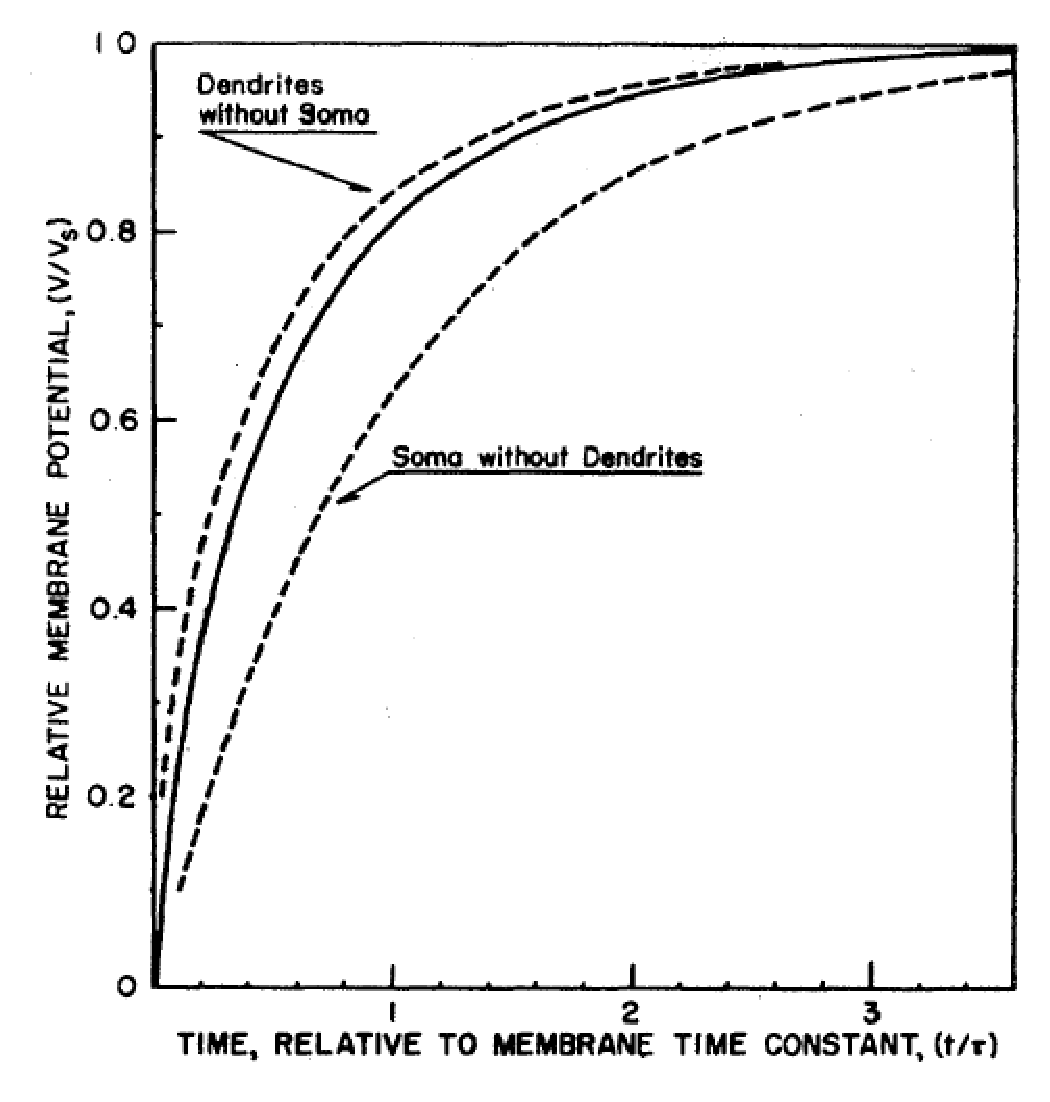
\includegraphics[height=5cm,
    angle=0]{./images/potential_soma.eps}}
  \caption{Membrane potential transient measured at soma and origins
    of dendrites (when constant current is applied uniformly across
    the soma membrane)}
\label{fig:soma_potential}
\end{figure}


% There is a difference in the time constants between that of soma
% membrane and that of synaptic potential decay.

However, neurons do have dendrites. In motoneuron there are several
large dendrites, thus a significant portion of the applied current
must spread (electrotonically) along these several dendrites. As a
result, it will change the time course of the soma membrane potential.

Under the theoretical assumptions that
\begin{enumerate}
\item All dendrites is big relative to the soma size,
\item They have same membrane time constant $\tau$
\item They may be represented as cylinders with infinite length. 
\end{enumerate}
This is called ``dendrites without soma''. The curve (upper dashed
curve) is then slightly different from the true curve (solid
curve). It is not simple exponential, as the time to reach 
\begin{itemize}
\item half of the steady value $V_s$ is one-third of the time
\item 90\% of $V_s$ is three-fifths of the time
\end{itemize}
found in the lower dash curve.


% \begin{eqnarray}
%   \label{eq:450}
%   V/V_s = \text{erf} \sqrt{t/\tau}
% \end{eqnarray}
So, the solid middle curve represents an intermediate relation between
the dendrite network and some, and more practical. However, it needs
the assumption that 
\begin{itemize}
\item the soma and the dendrites have the same membrane time
  constant. 
\item the membrane potential at any moment is uniform over the soma
  surface, up to and including the origins of the dendrites. 
\item the dendrites can be treated as a cylinders or a structure which
  branch exponentially.
\end{itemize}
As these assumptions still underestimate the size and number of
dendrites, thus, it is believed that the time course of the soma will
lie between the two upper curves (for many motoneurons).


\subsection{Spread of current from soma to dendritic trees}
\label{sec:spread-current-from}

The theory is general and can be applied to many types of neurons with
many types of dendritic trees; it is also relevant to the diffusion of
material in neurons. The $3/2$ power of dendritic trunk diameter is
shown to be a fundamental index of dendritic size~\citep{rall1959bdt}. 
\begin{figure}[hbt]
  \centerline{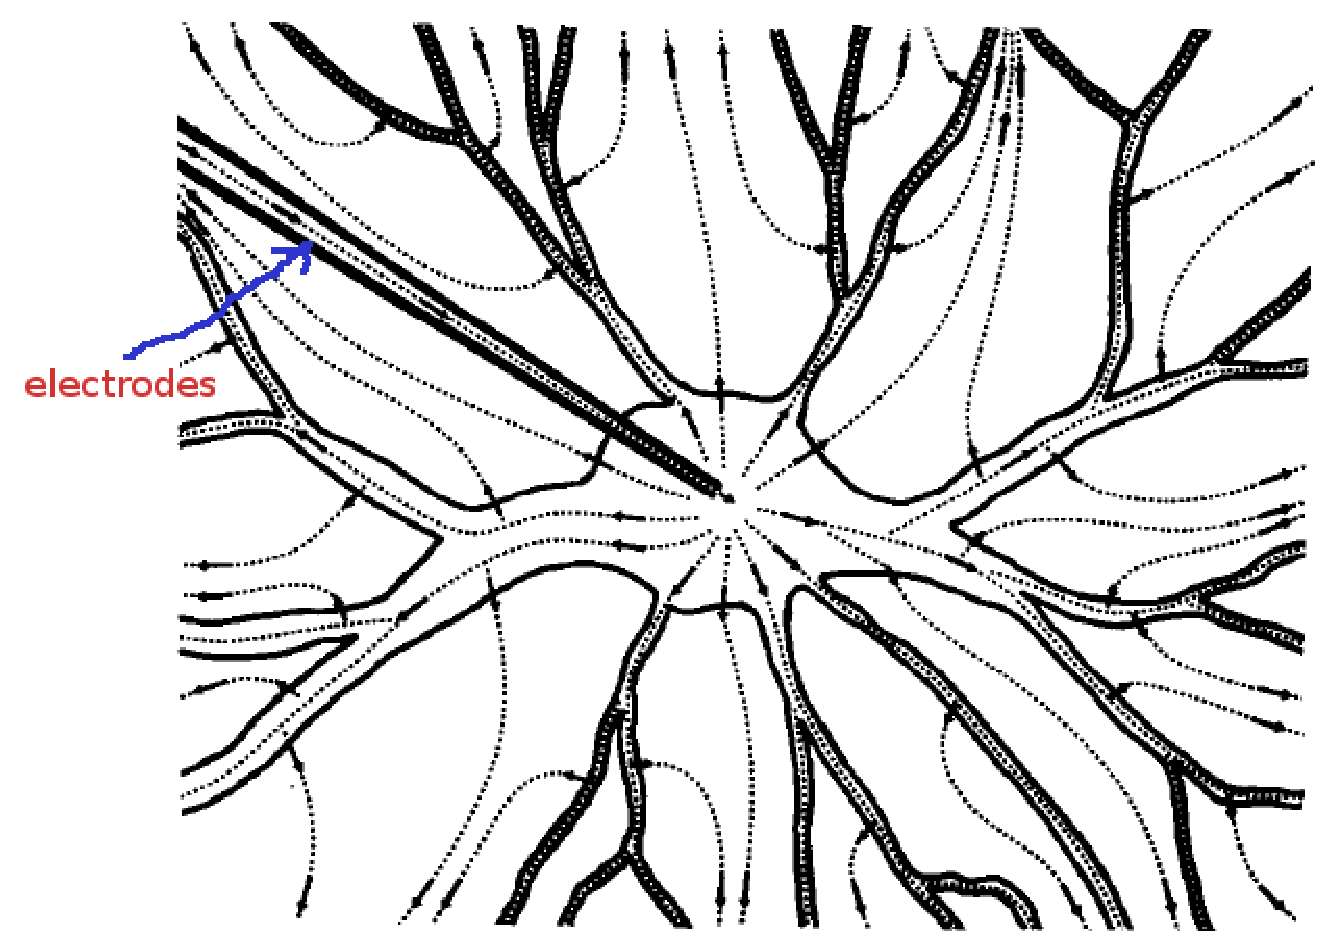
\includegraphics[height=5cm,
    angle=0]{./images/somacurrent_flow.eps}}
\caption{Diagram illustrating the flow of current from the
  microelectrode whose tips penetrate the soma of a neuron}
\label{fig:current_flow}
\end{figure}

The total flows is determined by the electric and geometric factors. 
\begin{itemize}
\item electric factors (for steady state conditions): membrane
  resistivity and specific resistivities of the intracellular and
  extracellular media, membrane capacity
\item geometric factors: size of neuron soma, size and taper of all
  dendrite trunks, as well as amount and extent of dendrite
  branching. 
\end{itemize}

The very first models, ``standard motoneuron'' of Eccles
\citep{eccles1957pnc} assumed the dendrites as cylinders of infinite
length; a cat motoneurons with 6 such cylinders of diameter
$d=5\mu$m. However, such model and its derivatives underestimated
the dendritic contribution by a significant amount.


In motoneurons, the synaptic activation cause the dendrite to undergo
a brief active phase of depolarization. This depolarization was
assumed to undergo a ``passive'' decay having exponential time
constant about $\tau = R_mC_M = 4$ ms on average (with a range from 3
to 5ms in cat motoneurons). This active phase was believed to result
from a large non-selective increase of the ionic permeability of the
motoneuron membrane~\citep{rall1960mpt}.

{\bf The word ''passive'' is used to imply that the membrane resistance,
  capacity, and electromotive forces all remain constant at their
  physiological resting values.}

The membranet ime constantc an
be: estimated as being the time required
for the experimentalt ransientst o reach
about 82 percent of the final steady
value.

$R_m=2000$ Ohm.cm$^2$.

%%% Local Variables: 
%%% mode: latex
%%% TeX-master: "mainfile"
%%% End: 
